% Intended LaTeX compiler: pdflatex
\documentclass[10pt,a4paper,UTF8]{article}
\usepackage{zclorg}
\usepackage{tikztheorem}
\author{emacsun}
\date{}
\title{Thinking in Java chapter 9 多态}
\hypersetup{
 pdfauthor={emacsun},
 pdftitle={Thinking in Java chapter 9 多态},
 pdfkeywords={},
 pdfsubject={},
 pdfcreator={Emacs 25.2.1 (Org mode 9.0.9)},
 pdflang={English}}
\begin{document}

\maketitle
\tableofcontents
\titlepic{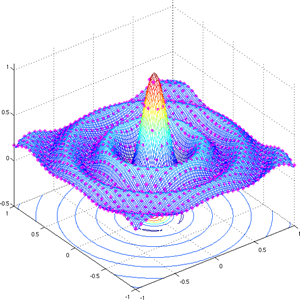
\includegraphics[scale=0.25]{../../img/sinc.PNG}}

\section{简介}
\label{sec:org5d6d00b}


继数据抽象(data abstraction)和继承( Inheritance )之后,多态(polymorphism)是 Java 语言支持的又一重要特性。

使用多态,可以针对同一个操作输入多种类型的数据。多态指的是同一操作支持多中数据类型。这在动态语言中显得尤为明显,比如 \texttt{Python} 。在 \texttt{Java} 中,我们也碰到过多态的例子,比如对于 \texttt{+} 如果我们 \texttt{1+2} 我们期待输出的结果是 \texttt{3} ,此时, \texttt{+} 的功能是数学里的加法运算,但是对于 \texttt{'a' + 'bc'} 这样的运算,我们希望输出的是 \texttt{'abc'} 也就是字符串的级联。这个小例子体现了 \texttt{+} 的多种形态。

多态往往和动态绑定等价。在很多地方 polymorphism 和 dynamic binding , late binding, runtime binding 相提并论。
\section{重访 upcasting}
\label{sec:orge821caa}


我们知道通过继承,一个对象的类型可以是当前类(class),也可以是其父类。把一个对象的类型当作其父类来处理就叫做 upcasting. 但是通过下面的这个例子,我们就会看到 upcasting 会导致一个问题。

这是一个关于音乐的例子,由于多个类都要用到 Notes,比如 C 小调之类的专有名词,我们首先建立一个 \texttt{enum}

\lstset{language=C,label= ,caption= ,captionpos=b,firstnumber=1,numbers=left}
\begin{lstlisting}
//: polymorphism/music/Note.java
// Notes to play on musical instruments.
package polymorphism.music;

public enum Note {
    MIDDLE_C, C_SHARP, B_FLAT; // Etc.
} ///:~
\end{lstlisting}

然后, \texttt{Wind} 是一个乐器 \texttt{Instrument} 。 \texttt{Wind} 类就继承自 \texttt{Instrument} 类。

\texttt{Instrument} 类:
\lstset{language=C,label= ,caption= ,captionpos=b,firstnumber=1,numbers=left}
\begin{lstlisting}
//: polymorphism/music/Instrument.java
package polymorphism.music;
import static net.mindview.util.Print.*;

class Instrument {
  public void play(Note n) {
    print("Instrument.play()");
  }
}
 ///:~
\end{lstlisting}
\texttt{Wind} 类:
\lstset{language=C,label= ,caption= ,captionpos=b,firstnumber=1,numbers=left}
\begin{lstlisting}
//: reusing/Wind.java
// Inheritance & upcasting.
package polymorphism.music;


// Wind objects are instruments
// because they have the same interface:
public class Wind extends Instrument {
  public void play(Note n){
   System.out.println("Wind.play" + n);
  }
} ///:~
\end{lstlisting}
最后是 \texttt{Music} 类:
\lstset{language=C,label= ,caption= ,captionpos=b,firstnumber=1,numbers=left}
\begin{lstlisting}
//: polymorphism/music/Music.java
// Inheritance & upcasting.
package polymorphism.music;

public class Music {
  public static void tune(Instrument i) {
    // ...
    i.play(Note.MIDDLE_C);
  }
  public static void main(String[] args) {
    Wind flute = new Wind();
    tune(flute); // Upcasting
  }
} /* Output:
Wind.play() MIDDLE_C
*///:~
\end{lstlisting}
注意, \texttt{Music} 类的 \texttt{Music.tune}  方法接受了一个 \texttt{Instrument} 类型的对象。这说明任何从 \texttt{Instrument} 类继承下来的类的对象都可以送给 \texttt{Music.tune}. 在 \texttt{Music} 的 \texttt{main} 函数中,我们送给 \texttt{tune} 的就是 \texttt{Wind} 类型的对象。这是没有问题的,因为 \texttt{Wind} 类继承自 \texttt{Instrument} 类。在这里,通过给 \texttt{tune} 函数送入 \texttt{Instrument} 类型的对象,而不是 \texttt{Wind} 类型的对象,我们节约了大量的代码量。想象一下,乐器有好多种,也就是从 \texttt{Instrument} 类可以继承下来很多对象。如果我们为每一个乐器都写一个 \texttt{tune} 函数,这将是多么无聊的事情。

看如下无聊的代码:
\lstset{language=C,label= ,caption= ,captionpos=b,firstnumber=1,numbers=left}
\begin{lstlisting}
//: polymorphism/music/Music2.java
// Overloading instead of upcasting.
package polymorphism.music;
import static net.mindview.util.Print.*;

class Stringed extends Instrument {
  public void play(Note n) {
    print("Stringed.play() " + n);
  }
}

class Brass extends Instrument {
  public void play(Note n) {
    print("Brass.play() " + n);
  }
}

public class Music2 {
  public static void tune(Wind i) {
    i.play(Note.MIDDLE_C);
  }
  public static void tune(Stringed i) {
    i.play(Note.MIDDLE_C);
  }
  public static void tune(Brass i) {
    i.play(Note.MIDDLE_C);
  }
  public static void main(String[] args) {
    Wind flute = new Wind();
    Stringed violin = new Stringed();
    Brass frenchHorn = new Brass();
    tune(flute); // No upcasting
    tune(violin);
    tune(frenchHorn);
  }
} /* Output:
Wind.play() MIDDLE_C
Stringed.play() MIDDLE_C
Brass.play() MIDDLE_C
*///:~
\end{lstlisting}
上面的代码可以工作,但是这个代码结构有一个致命的问题:你必须为每一个乐器编写 \texttt{tune} 函数。 那么,如果能够只写一次 \texttt{tune} 方法,且送入的对象是 \texttt{Instrument} 类型,而不是 \texttt{Instrument} 的任一子类,岂不是更好?也就是说,在使用 \texttt{tune} 方法的时候,我们如果忘记 \texttt{tune} 的参数类型岂不是更好?这就是多态带来的福利。
\section{纠结}
\label{sec:org9adbf17}


现在,我们有一个问题, \texttt{Java} 在编译的过程中怎么知道 \texttt{Instrument} 类指向的是 \texttt{Wind} 而不是 \texttt{Brass} 或者 \texttt{Stringed} 类?答案是:编译器不知道。为理解这个问题,我们探讨 \texttt{binding} 的原理。

\subsection{方法调用 \texttt{binding}}
\label{sec:org9e01083}

把方法调用和方法本身连接起来的过程叫做 \texttt{binding} 。程序执行之前的 binding 叫做 early binding (可能由编译器和链接器来完成)。 \texttt{C} 语言种的 binding 都是 early binding。但是,我们前面的例子告诉我们 \texttt{Java} 中, \texttt{binding} 的方式有些不一样。因为编译器不知道到底该调用哪个方法。所以 \texttt{Java} 中的 binding 方法是所谓的 late binding .意味着 binding 发生在程序运行时。late binding 也叫做 dynamic binding 或者 runtime binding。

Java 中除了 \texttt{static} 和 \texttt{final} 方法外,所有的方法都是 \textbf{late binding} .这意味着,你不需要显示的为某个方法指示用什么 binding 方式。Java 已经帮你安排好了。所有的 \texttt{private} 方法都是 \texttt{final} 类型的。指定一个方法为 \texttt{final} 意味着,你不想这个方法动态绑定。这样做的一个好处是编译器会编译出更高效的代码。但是,你不能因为性能的借口,到处使用 \texttt{final} ,你应该处于设计的原因使用 \texttt{final} ,毕竟使用 \texttt{final} 带来的性能提升没有那么多。

\subsection{正确的行为}
\label{sec:org55291da}

一旦知晓 Java 的动态绑定,我们就可以写出支持多态的漂亮代码。你的代码针对的类型不只是当前类,当前类的父类,父类的父类的对象都可以作为参数。这在 \texttt{Python} 中也有明显的体现(Python 是完全动态的语言)。 我们使用一个经常用到的例子来阐述与 动态绑定相关的概念。
\begin{figure}[htbp]
\centering
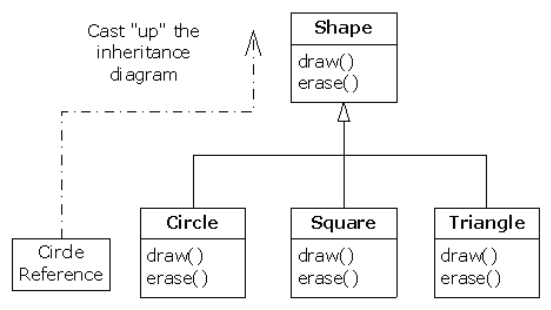
\includegraphics[width=0.6\textwidth]{../../img/computer_TIJ/20170730shape.png}
\caption{\label{fig:org9a003fa}
动态绑定}
\end{figure}

根据上图:
\lstset{language=java,label= ,caption= ,captionpos=b,numbers=none}
\begin{lstlisting}
Shape s = new Circle();
\end{lstlisting}
这个语句生成了 \texttt{Circle} 对象,生成的结果转换成了 \texttt{Shape} 类型。貌似,这是一个错误,毕竟我们把一种类型的对象转换成了另一种类型。但是,这是可以的,因为 \texttt{Circle} 类继承自 \texttt{Shape} . 问题来了,
\lstset{language=java,label= ,caption= ,captionpos=b,numbers=none}
\begin{lstlisting}
s.draw();
\end{lstlisting}
调用的是哪个函数?你可能会认为调用的是 \texttt{Shape} 的 \texttt{draw()} 函数,因为 \texttt{s} 被转换成了 \texttt{Shape} 类型。但是,这里调用的是 \texttt{Circle.draw()} . 为甚么?因为多态。

接下来,看代码,首先是 \texttt{Shape} 类:
\lstset{language=java,label= ,caption= ,captionpos=b,firstnumber=1,numbers=left}
\begin{lstlisting}
//: polymorphism/shape/Shape.java
package polymorphism.shape;

public class Shape {
  public void draw() {}
  public void erase() {}
} ///:~
\end{lstlisting}
\texttt{Circle} 类:
\lstset{language=java,label= ,caption= ,captionpos=b,firstnumber=1,numbers=left}
\begin{lstlisting}
//: polymorphism/shape/Circle.java
package polymorphism.shape;
import static net.mindview.util.Print.*;

public class Circle extends Shape {
  public void draw() { print("Circle.draw()"); }
  public void erase() { print("Circle.erase()"); }
} ///:~
\end{lstlisting}
\texttt{Square} 类:
\lstset{language=java,label= ,caption= ,captionpos=b,firstnumber=1,numbers=left}
\begin{lstlisting}
//: polymorphism/shape/Square.java
package polymorphism.shape;
import static net.mindview.util.Print.*;

public class Square extends Shape {
  public void draw() { print("Square.draw()"); }
  public void erase() { print("Square.erase()"); }
} ///:~
\end{lstlisting}
\texttt{Triangle} 类:
\lstset{language=java,label= ,caption= ,captionpos=b,firstnumber=1,numbers=left}
\begin{lstlisting}
//: polymorphism/shape/Triangle.java
package polymorphism.shape;
import static net.mindview.util.Print.*;

public class Triangle extends Shape {
  public void draw() { print("Triangle.draw()"); }
  public void erase() { print("Triangle.erase()"); }
} ///:~
\end{lstlisting}
随机生成形状类:
\lstset{language=java,label= ,caption= ,captionpos=b,firstnumber=1,numbers=left}
\begin{lstlisting}
//: polymorphism/shape/RandomShapeGenerator.java
// A "factory" that randomly creates shapes.
package polymorphism.shape;
import java.util.*;

public class RandomShapeGenerator {
  private Random rand = new Random(47);
  public Shape next() {
    switch(rand.nextInt(3)) {
      default:
      case 0: return new Circle();
      case 1: return new Square();
      case 2: return new Triangle();
    }
  }
} ///:~
\end{lstlisting}
调用以上代码:
\lstset{language=java,label= ,caption= ,captionpos=b,firstnumber=1,numbers=left}
\begin{lstlisting}
//: polymorphism/Shapes.java
// Polymorphism in Java.
import polymorphism.shape.*;

public class Shapes {
  private static RandomShapeGenerator gen =
    new RandomShapeGenerator();
  public static void main(String[] args) {
    Shape[] s = new Shape[9];
    // Fill up the array with shapes:
    for(int i = 0; i < s.length; i++)
      s[i] = gen.next();
    // Make polymorphic method calls:
    for(Shape shp : s)
      shp.draw();
  }
} /* Output:
Triangle.draw()
Triangle.draw()
Square.draw()
Triangle.draw()
Square.draw()
Triangle.draw()
Square.draw()
Triangle.draw()
Circle.draw()
*///:~
\end{lstlisting}
基类 \texttt{Shape} 构建了所有子类的函数接口:所有的子类都可以被 \texttt{draw} 和 \texttt{erase} 。 \texttt{RandomShapeGenerator} 是一个形状工厂,随机生成形状对象,并保存在 \texttt{s} 中。每一个类对象是 \texttt{Circle} \texttt{Square} 或者 \texttt{Triangle} 中的一个,但是在 \texttt{return} 的时候, \texttt{upcast} 成为 \texttt{Shape} 类对象。因此当调用 \texttt{next()} 时,返回的永远是 \texttt{Shape} 类对象。

\texttt{main()} 函数通过调用 \texttt{RandomShapeGenerator.next()} 生成了 9 个 \texttt{Shape} 类对象,保存在 \texttt{s} 中。在这个时候,你知道你有一个 \texttt{Shape} 的数组,但是你不知道,生成的到底时 \texttt{Circle} \texttt{Square} 还是 \texttt{Triangle} 。但是,当你逐个调用 \texttt{draw()} 函数的时候,奇妙的事情发生了, \texttt{Java} 居然可以知道每一个 \texttt{Shape} 该执行哪一个 \texttt{draw()} 这个就是多态。
\end{document}
